%%%%%%%%%%%%%%%%%%%%%%%%%%%%%%%%%%%%%%%%%
% Short Sectioned Assignment LaTeX Template Version 1.0 (5/5/12)
% This template has been downloaded from: http://www.LaTeXTemplates.com
% Original author:  Frits Wenneker (http://www.howtotex.com)
% License: CC BY-NC-SA 3.0 (http://creativecommons.org/licenses/by-nc-sa/3.0/)
%%%%%%%%%%%%%%%%%%%%%%%%%%%%%%%%%%%%%%%%%

%----------------------------------------------------------------------------------------
%	PACKAGES AND OTHER DOCUMENT CONFIGURATIONS
%----------------------------------------------------------------------------------------

\documentclass[paper=a4, fontsize=11pt]{scrartcl} % A4 paper and 11pt font size

% ---- Entrada y salida de texto -----

\usepackage[T1]{fontenc} % Use 8-bit encoding that has 256 glyphs
\usepackage[utf8]{inputenc}

% ---- Idioma --------

\usepackage[spanish, es-tabla]{babel} % Selecciona el español para palabras introducidas automáticamente, p.ej. "septiembre" en la fecha y especifica que se use la palabra Tabla en vez de Cuadro

% ---- Otros paquetes ----

\usepackage{amsmath,amsfonts,amsthm} % Math packages
\usepackage{graphics,graphicx, floatrow} %para incluir imágenes y notas en las imágenes
\usepackage{graphics,graphicx, float} %para incluir imágenes y colocarlas
\usepackage{hyperref} % url in references
\usepackage{listings}
\usepackage{color}
\definecolor{grey}{gray}{0.9}

% Para hacer tablas comlejas
\usepackage{multirow}
\usepackage{threeparttable}

\usepackage{fancyhdr} % Custom headers and footers
\pagestyle{fancyplain} % Makes all pages in the document conform to the custom headers and footers
\fancyhead{} % No page header - if you want one, create it in the same way as the footers below
\fancyfoot[L]{} % Empty left footer
\fancyfoot[C]{} % Empty center footer
\fancyfoot[R]{\thepage} % Page numbering for right footer
\renewcommand{\headrulewidth}{0pt} % Remove header underlines
\renewcommand{\footrulewidth}{0pt} % Remove footer underlines
\setlength{\headheight}{13.6pt} % Customize the height of the header

\numberwithin{equation}{section} % Number equations within sections (i.e. 1.1, 1.2, 2.1, 2.2 instead of 1, 2, 3, 4)
\numberwithin{figure}{section} % Number figures within sections (i.e. 1.1, 1.2, 2.1, 2.2 instead of 1, 2, 3, 4)
\numberwithin{table}{section} % Number tables within sections (i.e. 1.1, 1.2, 2.1, 2.2 instead of 1, 2, 3, 4)

\setlength\parindent{0pt} % Removes all indentation from paragraphs - comment this line for an assignment with lots of text

\newcommand{\horrule}[1]{\rule{\linewidth}{#1}} % Create horizontal rule command with 1 argument of height

\usepackage{textcomp}
\usepackage{hyperref}

%----------------------------------------------------------------------------------------
%	DATOS
%----------------------------------------------------------------------------------------

\newcommand{\myName}{Francisco Javier Bolívar Lupiáñez}
\newcommand{\myColleageName}{Juan Pablo González Casado}
\newcommand{\myDegree}{Máster en Ingeniería Informática}
\newcommand{\myFaculty}{E. T. S. de Ingenierías Informática y de Telecomunicación}
\newcommand{\myDepartment}{Ciencias de la Computación e Inteligencia Artificial}
\newcommand{\myUniversity}{\protect{Universidad de Granada}}
\newcommand{\myLocation}{Granada}
\newcommand{\myTime}{\today}
\newcommand{\myTitle}{Práctica 2}
\newcommand{\mySubtitle}{Clasificación de Imágenes}
\newcommand{\mySubject}{Sistemas Inteligentes para la Gestión de la Empresa}
\newcommand{\myYear}{2016-2017}

%----------------------------------------------------------------------------------------
%	PORTADA
%----------------------------------------------------------------------------------------


\title{	
	\normalfont \normalsize 
	\textsc{\textbf{\mySubject \space (\myYear)} \\ \myDepartment} \\[20pt] % Your university, school and/or department name(s)
	\textsc{\myDegree \\[10pt] \myFaculty \\ \myUniversity} \\[25pt]
	\horrule{0.5pt} \\[0.4cm] % Thin top horizontal rule
	\huge \myTitle: \mySubtitle \\ % The assignment title
	\horrule{2pt} \\[0.5cm] % Thick bottom horizontal rule
	\normalfont \normalsize
}

\author{
	\myName \\ 
	\myColleageName \\ \\ 
	\small Kaggle: \texttt{EchaEquipos} \\
	\small Posición: 195, Puntuación: 0.80378 \\ 
}

\date{\myTime} % Incluye la fecha actual
%----------------------------------------------------------------------------------------
%	INDICE
%----------------------------------------------------------------------------------------

\begin{document}
	
\definecolor{light-gray}{gray}{0.95}
	
\lstset {
	basicstyle=\scriptsize,
	frame=single,
	backgroundcolor=\color{grey}
}

\lstdefinestyle{R}{
	frame=single,
	numbers=left,
	language=R,
	basicstyle=\tiny\ttfamily,
	keywordstyle=\bfseries,
	commentstyle=\itshape,
	identifierstyle=\bfseries,
}
	
\setcounter{page}{0}

\maketitle % Muestra el Título
\thispagestyle{empty}

\newpage %inserta un salto de página

\tableofcontents % para generar el índice de contenidos

%\listoftables
%\listoffigures

\newpage

%----------------------------------------------------------------------------------------
%	DOCUMENTO
%----------------------------------------------------------------------------------------

\section{Exploración de datos}

Los datos que tenemos son una serie de imágenes a color con un tamaño de 3096 x 4128 y un peso aproximado que ronda de entre 2.5 a 7.5 MB.
\\ \\
Estas imágenes son fotos de cérvix femenina (parte inferior del útero) echadas desde distintas distancias y ángulos.
\\ \\
En el caso de las imágenes de \textit{train} las tenemos estructuradas en tres directorios distintos (\texttt{Type\_1}, \texttt{Type\_2} y \texttt{Type\_3}), uno por cada clase. En el caso de las imágenes de \textit{test} las tenemos todas en un solo directorio pues desconocemos el tipo de cada uno y es que ese será el objetivo de la práctica: clasificar cada una de estas 512 imágenes en los tres tipos distintos.
\\ \\
El conjunto de datos de \textit{train} consta 1481 imágenes, no obstante Kaggle proporciona más imágenes adicionales para aumenta a 7004 el número de imágenes para entrenar nuestros modelos.

\subsection{Dataset no balanceado}

Lo primero que podemos observar es que tanto el conjunto básico (Figura \ref{fig:num-images-train-dataset}) como el que incluye las imágenes adicionales (Figura \ref{fig:num-images-train-extra-dataset}) se encuentran desequilibrados con pocas imágenes del tipo 1 y muchas de los tipos 2 y 3. Esto es algo que tendremos que tener muy en cuenta a la hora de realizar el preprocesamiento de datos.

\begin{figure}[H]
	\centering
	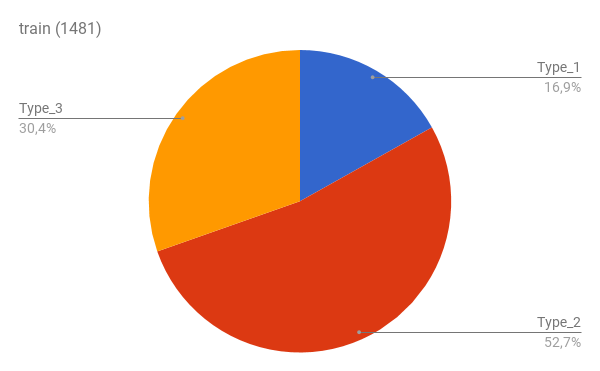
\includegraphics[width=12cm]{img/num-images-train-dataset}
	\caption{Porcentaje de imágenes de cada tipo para el \textit{dataset} básico}
	\label{fig:num-images-train-dataset}
\end{figure}

\begin{figure}[H]
\centering
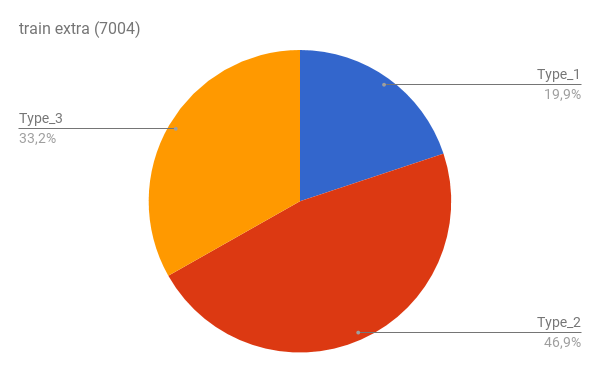
\includegraphics[width=12cm]{img/num-images-train-extra-dataset}
\caption{Porcentaje de imágenes de cada tipo para el \textit{dataset} que incluye las imágenes adicionales}
\label{fig:num-images-train-extra-dataset}
\end{figure}

\subsection{Imágenes que no corresponden a un cérvix}

Además, a la hora de explorar cada uno de estos datos, nos encontramos con imágenes que no correspondían a un cérvix o se encontraban demasiado borrosas (Figura \ref{fig:no-cervix-image}). Obviamente, en el posterior proceso de preprocesamiento de datos se eliminarán para que no agreguen ningún tipo de ruido a nuestro modelo.

\begin{figure}[H]
	\centering
	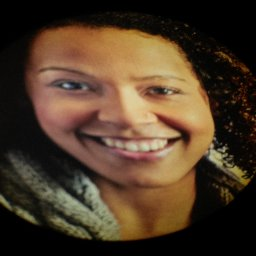
\includegraphics[width=3.5cm]{img/3086}
	
\includegraphics[width=3.5cm]{img/4065}
	
\includegraphics[width=3.5cm]{img/4533}
	
\includegraphics[width=3.5cm]{img/4367}
	\caption{Ejemplos de imágenes que se encuentran en el \textit{dataset} pero no corresponden a un cérvix o se encuentran demasiado borrosas}
	\label{fig:no-cervix-image}
\end{figure}

\section{Preprocesamiento de datos}

Como comenté en la sección anterior. Lo primero que hicimos fue borrar todas las fotos que no correspondían a cérvix o estaban demasiado borrosas. Después de esto nos planteamos realizar \textit{data augmentation}. Para ello realizamos varios \textit{scripts} en R con los que realizábamos operaciones de rotación y volteo para generar hasta ocho imágenes más por cada imagen. No obstante no llegamos a utilizarlos por problemas en memoria en nuestros equipos, y es que ni siquiera podíamos leer a un tamaño de 224 x 224 (necesario para \textit{fine-tuning}) las 7000 imágenes de Kaggle.
\\ \\
Como hacía falta reducir el número de imágenes se aprovechó para hacer \textit{undersampling} y balancear el conjunto de datos (Figura \ref{fig:num-images-train-extra-balanced-dataset}). No se equilibró totalmente pero se hizo lo suficiente como para que dejase de ser un conjunto de datos desequilibrado.

\begin{figure}[H]
	\centering
	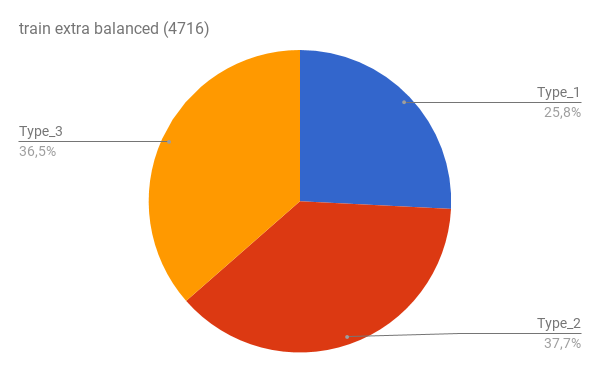
\includegraphics[width=12cm]{img/num-images-train-extra-balanced-dataset}
	\caption{Porcentaje de imágenes de cada tipo para el \textit{dataset} que incluye las imágenes adicionales al que posteriormente se le ha realizado \textit{undersampling} para balancearlo.}
	\label{fig:num-images-train-extra-balanced-dataset}
\end{figure}

El conjunto de datos final cuenta con 4716 imágenes (1217 del primer tipo, 1780 del segundo y 1719 del tercero).

\section{Técnicas de clasificación}

\subsection{\textit{Learning from scratch}}

Lala

\subsection{\textit{Fine-tuning}}

Lala

\section{Presentación y discusión de resultados}

Lala

\section{Conclusiones y trabajo futuro}

Lala

\section{Listado de soluciones}

Lala

%----------------------------------------------------------------------------------------
%	REFERENCIAS
%----------------------------------------------------------------------------------------

\newpage

\bibliography{referencias} %archivo referencias.bib que contiene las entradas 
\bibliographystyle{plain} % hay varias formas de citar

\end{document}